\newcommand{\decision}{\operatornamewithlimits{\gtrless}}
\newcommand{\argmax}{\operatornamewithlimits{argmax}}
\newcommand{\argmin}{\operatornamewithlimits{argmin}}

\chapter{Quantity modulation}
\label{c:qm}

\section{Introduction}
 In this chapter, we study the communication between two nano-machines with information embedded in different molecular quantity~\cite{Andrew1}. In the rest of this chapter, we call this kind of modulation as quantity modulation (QM). It is known that in diffusion-based molecular communications, molecules are emitted by the transmitter and move towards the receiver following the laws of molecule diffusion. Recent studies on diffusion-based molecular communications often model the statistical behavior of molecule diffusion as a Brownian motion~\cite{brown}. Due to the random nature of Brownian motions, molecules that released earlier by TN may arrive late. Therefore, messages carried in current molecules may be interfered by those delayed molecules that were transmitted earlier. 
This phenomenon is known as the ISI effect in diffusion-based molecular communications. A brief discussion about this effect can be found in~\cite{ISI_concen} and~\cite{delaySelector}.

There are lots of ways to design filters to eliminate the effect of ISI in conventional communication such as linear equalizer, adaptive equalizer and decision-feedback equalizer~\cite{commSysEng}. However, both linear equalizer and adaptive equalizer do not work well in molecular communication due to time-varying channel response.
 In this chapter, we utilize the concept of decision feedback and introduce a method to mitigate the effect of ISI.

The rest of this chapter is organized as follows: In Section II, we introduce the settings of a binary QM molecular communication system in details. We also describe the characteristics and the mathematical model of a Brownian motion channel. Section III focuses on deriving the decision rule for one-shot transmission of the binary QM system and extending it to the M-ary transmission case. In Section IV, we consider serial transmission and take ISI effect into account. ISI cancellation method is also described in this section. Numerical results are shown in Section V. Finally, we make conclusions in Section VI.

\section{System model}
In this section, we first give a general model for transmitter, receiver, and channel in molecular communication. We then describe a QM system of $M$ quantity levels ($M$-ary modulation) bearing $\log_2M$ information bits, which will be used later to apply our ISI cancellation method.

\subsection{Transmitter}
Fig.~\ref{fig:machine} illustrates a transmitter nano-machine TN transmitting molecules to a receiver nano-machine RN. When TN receives the information (e.g. bit pattern) to be transmitted, it starts storing certain number of molecules in a vesicle (i.e. container that stores molecules) and release these molecules simultaneously into the environment. The number of released molecules differs according to the transmitting information. In practical situations, molecules leaves the vesicle with random timing which is discussed in~\cite{secrete_phy}. In this paper, we simply assume that molecules exit the vesicle simultaneously.

\begin{figure}[htb]
\centering
\includegraphics[width=3.5in, keepaspectratio]{QM/machine.eps}
\caption{Transmission from TN to RN through a fluid medium.} \label{fig:machine}
\end{figure}

\subsection{Receiver}
RN is located at a position $d > 0$ apart from TN. There are several receptors capturing molecules on RN. RN counts the number of molecules it captures and perform detection according to the number. We assume the molecules can be perfectly captured by the receptors and RN does not have counting errors. Furthermore, once a molecule arrives at RN, it will be removed from the communication medium.

\subsection{Channel}
Consider a fluid medium between TN and RN with positive drift velocity $v$. The molecules are all constrained to move in a one-dimensional space. We assume that the trajectory of emitted molecules can be modeled with independent Brownian motions\cite{brown}.
Let $X$ denote the random variable representing the first hitting time (i.e. time difference between releasing and capturing) of a molecule. If $v > 0$, it can be shown that the probability density function (pdf) of $X$ is given by the inverse Gaussian (IG) distribution \cite{Chhikara:1989:IGD:73944}

\begin{eqnarray}
f_X(x) = \left\{\begin{array}{ll}
                 \sqrt{\dfrac{\lambda}{2\pi x^3}}\exp \left\{ -\dfrac{\lambda (x-\mu)^2}{2\mu^2 x} \right\}, & \mbox{$x>0$,}
                 \\
                 0, & \mbox{$x \leq 0$,}
                \end{array} \right. \label{IG_PDF}
\end{eqnarray}
\begin{eqnarray}
\mu = \dfrac{d}{v}\text{\ and\ } \lambda = \dfrac{d^2}{2D},\nonumber
\end{eqnarray}
where $D$ denotes the diffusion coefficient which is given by
\begin{eqnarray}
D = \dfrac{k_BT}{6\pi n r} \nonumber
\end{eqnarray}
where $k_B$ is the Boltzmann constant, $T$ is the temperature, $n$ is the viscosity of the fluid medium, and $r$ is the radius of molecule. For simplicity,
 we assume that the radii for all molecules are the same so that the diffusion coefficients are the same.

\subsection{QM system}
 Consider a time-slotted $M$-ary communication with signaling interval $T_s$, TN can release $M$ different quantities of molecules into the channel. Denote those $M$ quantities by $L_m$, where $m \in \{ 0,1,2,\cdots ,(M-1)\}$. Assume the \emph{a priori} probability for releasing $L_m$ molecules to be $q_m$. At the starting time of each transmission time slot, $L_m$ molecules are emitted simultaneously from the transmitter to indicate the transmission of a symbol. We assume perfect synchronization between the transmitter and the receiver. During each time slot, RN counts the total number of arriving molecules. An appropriate decision rule, proposed in Section~\ref{sec_detection}, is then applied to determine the transmitted data bit at the end of each time slot. The molecules which fail to arrive within the corresponding time slot become a source of interference, which will cause performance degradation to the detections of later coming symbols. Fig.~\ref{fig:modulation} is an example of QM system with $M=4$ and uniform quantity levels.

Perfect synchronization between TN and RN is assumed in this chapter, in chapter [ ] we provide a possible realization which is based on sending training molecular impulses and detecting the concentration peaks.

\begin{figure}[htb]
\centering
\includegraphics[width=5.5in, keepaspectratio]{QM/modulation.eps}
\caption{Illustration of quantity-based modulation scheme with $L_0=2$, $L_1=4$, $L_2=6$, $L_3=8$.} \label{fig:modulation}
\end{figure}

\section{Detection in one-shot transmission}
In this section, we discuss the detection rule of the system for one-shot transmission. The main contribution of our work is that we separate the ISI cancellation problem from the detection to achieve a more flexible and modularized design, which is different from previous works \cite{ICC_Meng}.

\subsection{Binary Detection}
 We define two hypotheses $H_0$ and $H_1$. $H_0$ is the hypothesis that $L_0$ molecules are transmitted (indicating bit $0$), and $H_1$ is the hypothesis that $L_1$ molecules are transmitted
 (indicating bit $1$).
 Denote the conditional pdf of the number of received molecules in a particular time slot, given that hypothesis $H_m$ is true, by $P(N=n | H_m)$, $m\in\{0,1\}$.
Using the inverse Gaussian pdf given in~\eqref{IG_PDF}, we define
the probabilities $p_j$ as:
\begin{eqnarray}
p_j = \int^{(j+1)T_s}_{j Ts} f_X(x)dx
\end{eqnarray}
for $j\in \{0,1,\cdots\}$, which is the probability that the traveling time of a molecule falls in the interval $[j T_s,(j+1)T_s]$,
where $j$ is the index of the time slots.
Define $Y_k$ to be the indicator random variable showing whether the $k$-th molecule emitted in a one-shot transmission arrives within $T_s$ given that $H_m$ is true. That is,
\begin{eqnarray}
Y_k = \left\{\begin{array}{ll}
                 1, & \mbox{if the $k$-th molecule arrives within $T_s$,} \\
                 \\
                 0, & \mbox{otherwise.} \\
                \end{array} \right.
\end{eqnarray}
Let $N$ be the random variable denoting the total number of molecules arriving at the receiver within a particular time slot. We have the following relation:
\begin{eqnarray}
P(N=n| H_m)=P(Y_1+Y_2+...+Y_{L_m}=n).
\end{eqnarray}
Given the number of the transmitted molecules, $N$ thus follows a binomial distribution with mean and variance as $L_m p_0$ and $L_m p_0(1-p_0)$, respectively. For large $L_m$, we approximate the binomial distribution by a Gaussian distribution with the knowledge of the mean and variance of $N$. Since it is difficult to manipulate directly with the binomial pdf, we will derive our detection threshold using Gaussian approximations instead.
Namely, we have
\begin{eqnarray}
P(N=n| H_m) \approx \dfrac{\exp
\left\{-\dfrac{(n-L_m p_0)^2}{2 L_m p_0(1-p_0)}\right\}}{\sqrt{2\pi L_m p_0(1-p_0)}}.
\end{eqnarray}
As a special case, the distributions of $N$ under two hypotheses can thus be obtained as
\begin{eqnarray}
P(N=n| H_0) \approx \dfrac{\exp\left\{-\dfrac{(n-L_0p_0)^2}{2L_0p_0(1-p_0)}\right\}}{\sqrt{2\pi L_0p_0(1-p_0)}}, \label{eq:h0}
\end{eqnarray}
\begin{eqnarray}
P(N=n| H_1) \approx \dfrac{\exp\left\{-\dfrac{(n-L_1p_0)^2}{2L_1p_0(1-p_0)}\right\}}{\sqrt{2\pi L_1p_0(1-p_0)}}. \label{eq:h1}
\end{eqnarray}
According to the conventional hypothesis testing theory \cite{vanTree, poor},
the decision rule can be expressed using the likelihood ratio $\Lambda(N)$ as
\begin{eqnarray}
\Lambda(N) =  \dfrac{P(N| H_1)}{P(N| H_0)} \decision ^{H_1}_{H_0} \dfrac{q_0}{q_1}.
\end{eqnarray}
If we assume equal \emph{a priori} probabilities $q_0=q_1=1/2$, due to the characteristic of Gaussian distribution shown in Fig.~\ref{fig:gaussian},  the decision rule can be further reduced to
\begin{eqnarray}
N \decision ^{H_1}_{H_0} \eta
\end{eqnarray}
for some threshold $\eta$,
where $\eta$ is the solution of the following equation:
\begin{eqnarray}
P(N = \eta | H_0) = P(N = \eta | H_1).
\end{eqnarray}
By~\eqref{eq:h0} and~\eqref{eq:h1}, we have
\begin{eqnarray}
\sqrt{ \dfrac{L_1}{L_0} } = \exp \left\{  \dfrac{(L_1-L_0) (\eta^2 - p_0^2L_0L_1) }{2 L_0 L_1 p_0(1-p_0)} \right\}.
\end{eqnarray}
Taking logarithms to both sides, the equation becomes
\begin{eqnarray}
\eta = \sqrt{ \dfrac{ L_1L_0\ln (L_1/L_0) }{L_1-L_0}p_0(1-p_0)+p_0^2L_0L_1 }. \label{eq:threshold}
\end{eqnarray}
In other words, if the received number of molecules is greater than the threshold $\eta$,  the receiver will determine $H_1$ as the hypothesis testing result; otherwise $H_0$ will be decided.

\begin{figure}[htb]
\centering
\includegraphics[width=5.5in, keepaspectratio]{QM/gaussian.eps}
\caption{Demonstration of the process of finding $\eta$ in a binary QM system, where $f$ is the conditional pdf of $N$ given $H_m$ is true.} \label{fig:gaussian}
\end{figure}

\subsection{M-ary Detection}
The detection rule can be extended to $M$-ary detection with only a few adjustments.
Suppose we have multiple hypotheses $H_m$ where $m \in \{ 0,1,2,\cdots,(M-1) \}$ which represent the transmission of $L_m$ molecules.
The goal is to decide which $\hat{m}$ we should choose.
The maximum \emph{a priori} (MAP)
detection rule is:
\begin{eqnarray}
\hat{m}(N) = \argmax_{m}P(N | H_m).
\end{eqnarray}
Due to the properties of Gaussian distribution, the above MAP detection rule can be simplified to pairwise comparisons between the ``neighboring'' conditional probability distributions.

To write down the expressions explicitly, we define a set of thresholds
$E = \{\eta_j \in [-\infty,\infty]\ :\ j = 0,1,2,\cdots,M \}$, and let $\eta_0 = -\infty$ and $\eta_M = \infty$.
For $j=1,2,\cdots,(M-1)$, $\eta_j$ can be obtained by solving the equations
\begin{eqnarray}
P(N=\eta_j | H_{j-1}) = P(N=\eta_j | H_j).
\end{eqnarray}
With the thresholds determined, the detection rule for $M$-ary transmission can be
expressed as
\begin{eqnarray}
\hat{m}(N) = \sum^{M-1}_{k=0}k \cdot u\left[-(N-\eta_k)(N-\eta_{k+1})\right].
\end{eqnarray}
where $u(\cdot)$ denotes the unit step function.

\subsection{Error Rate Analysis}
After the construction of the transmission and decision rules, we then analyze how it performs in terms of symbol or bit error rate. Consider a specific case for $M=2$ and $q_0 = q_1 = 1/2$. Denote the false alarm probability as $P_F$ and the missing probability as $P_M$. The error rate can be written as
\begin{eqnarray}
P_e = q_0P_F+q_1P_M=\dfrac{1}{2}(P_F+P_M). \label{eq:error}
\end{eqnarray}
From Fig.~\ref{fig:gaussian} and the decision rule derived in Subsection A, it can be shown that
\begin{eqnarray}
P_F = P(N>\eta | H_0) = Q\left( \dfrac{\eta-L_0p_0}{\sqrt{L_0 p_0 (1 - p_0)}} \right), \label{eq:falseAlarm}
\end{eqnarray}
\begin{eqnarray}
P_M = P(N < \eta | H_1) = Q\left( \dfrac{L_1p_0 - \eta}{\sqrt{ L_1 p_0 (1 - p_0)}} \right), \label{eq:missing}
\end{eqnarray}
where $Q(\cdot)$ denotes the Q-function.
By substituting~\eqref{eq:threshold} into equation~\eqref{eq:falseAlarm} and~\eqref{eq:missing}, we can evaluate the
error rate $P_e$ in~\eqref{eq:error}. Fig.~\ref{fig:error_rate} shows the comparison between our analysis and numerical results.

\begin{figure}[htb]
\centering
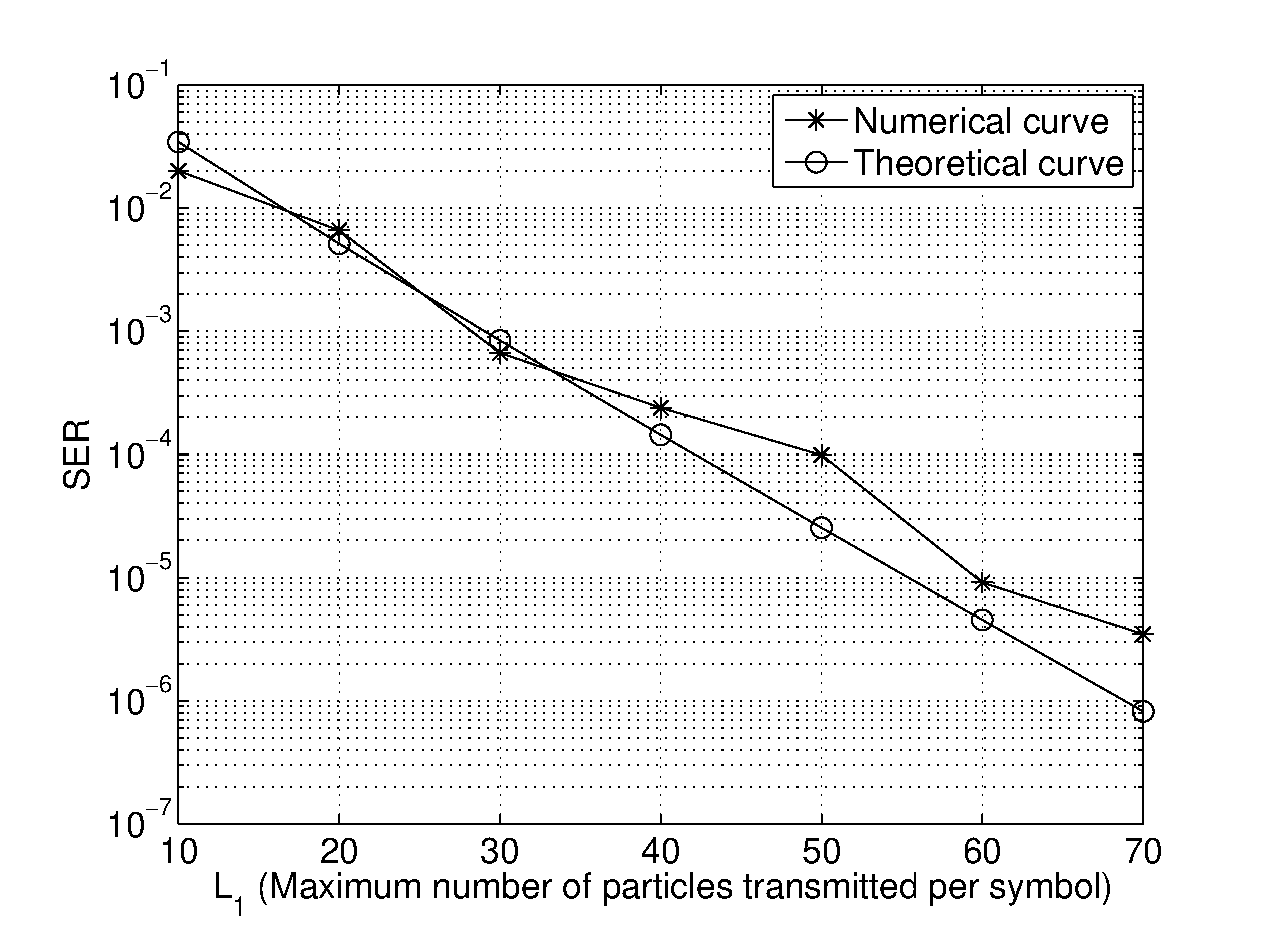
\includegraphics[width=5.5in, keepaspectratio]{QM/analysis_0329.eps}
\caption{Theoretical result versus numerical result for one-shot binary quantity-based modulation.} \label{fig:error_rate}
\end{figure}

\section{Serial transmision and ISI cancellation}
The above described QM molecular communication system seems to work already. However, in practical situations, we need to perform serial transmissions rather than one-shot transmission. Thus the ISI effect must be taken into account.
Our results show that if we do not modify our one-shot detection rule, the system performance will fall dramatically under serial transmission environments due to the severe ISI effect. To solve this problem, we propose a method to mitigate the ISI effect.

In order to mitigate the ISI effect, we first need an estimation of the number of the delayed molecules that come from former time slots. If we know the conditional probability distribution of the number of ISI molecules conditioned on the current received number, then we can estimate the ISI effect as the conditional mean.
However, the conditional distribution does not have a closed-form solution for inverse Gaussian random variables. Here we proposed another intuitive way to do this estimation.

First, we define ``memory-$\Gamma$ cancellation'' to mean that the ISI effect during the past $\Gamma$ time slots are taken into account when making decision. We first use memory-$1$ cancellation as a demonstrative example.
Suppose that the traveling time $\tau$ of each molecule can be described using an inverse Gaussian random variable with cumulative distribution function (cdf) $F_{\tau}(t)=\int_0^t f_X(x)dx$. Our proposed ISI cancellation method is: if the number of molecules received during the $(i-1)$-th time slot is $n_{i-1}$ and the decided transmission quantity level is $\hat{l}_{i-1}$, where $\hat{l}_{i-1} \in \{ L_0,L_1,\cdots,L_{M-1} \}$, we then subtract $\hat{l}_{i-1}\cdot[F_{\tau}(2T_s)-F_{\tau}(T_s)]$ (the \emph{a priori} expected received number in the $i$-th time slot from the $(i-1)$-th time slot) from $n_i$ before making the $i$-th decision. In other words, the actual number $\tilde{n}_i$ used in making decision is
\begin{eqnarray}
\tilde{n}_i = n_i - \hat{l}_{i-1}\cdot[F_{\tau}(2T_s)-F_{\tau}(T_s)].
\end{eqnarray}
Likewise, we can perform memory-$\Gamma$ cancellation if we have enough buffer at the receiver end to memorize temporarily the recently received numbers of molecules. More explicitly, denote the probabilities that a single transmitted molecule arrives during the time interval $[ j T_s,(j+1) T_s ]$ by $p_j$ for $j\in \mathbb{N} \cup \{0\}$ as before. If the decided transmission quantity level of the current time slot is $\hat{l}$, where $\hat{l} \in \{ L_0,L_1,\cdots,L_{M-1} \}$, then the received number of molecules $j$ time slots later should be subtracted by
$\hat{l} \cdot p_{j+1}$ before making decision. In other words, if the number of molecules received in $i$-th time slot is $n_i$, the actual number $\tilde{n}_i$ used in making decision is
\begin{eqnarray}
\tilde{n}_i = n_i - \sum^{\Gamma}_{j=1}\hat{l}_{i-j}p_{j+1}.
\end{eqnarray}
For binary QM systems, the decision rule can be written as
\begin{eqnarray}
\tilde{n}_i = n_i - \sum^{\Gamma}_{j=1}\hat{l}_{i-j}p_{j+1} \decision ^{H_1}_{H_0} \eta.
\end{eqnarray}
The extension to M-ary QM systems is straightforward.

\section{Numerical results}
In this section, we first discuss the binary and $M$-ary QM modulation systems with and without performing ISI cancellation.
After that, we make comparisons of the system performance under different time slot durations.

The number of molecules is one of the main resources utilized in molecular communications.
Analogous to the ``power'' concept in conventional communications, we need to take this number into account when comparing the system performances.
In the following subsections, we present the results under different maximum number of molecules allowed per symbol, and the quantity levels are uniformly spaced.
The simulation parameters are $d = 0.2\ cm$, drift velocity $v = 0.01\ cm/s$, diffusion coefficient $D = 0.05\ cm^2/s$ , and time slot duration $T_s = 5\ s$.

\subsection{SER comparison with and without ISI cancellation}
In Fig.~\ref{fig:binary_ser}, a binary transmission system with memory-1 and memory-2 cancellaion is considered. The SER drops from $0.04$ to $0.01$ when $L_1=30$, and drops from $10^{-2}$ to $10^{-4}$ when $L_1 = 90$. The improvement grows as $L_1$ increases, which means that by choosing $L_1$ properly, a reliable end-to-end transmission can be achieved. We also observe that even without ISI cancellation, the error rate will drop as $L_1$ increases. The reason is that the spacing between symbols is increased. However, as shown in Fig.~\ref{fig:4ary_ser}, it is not the case for the quaternary transmission system. It can be seen that even though $L_3$ becomes large, the error rate is still high without ISI cancellation, which means we cannot rely solely on increasing the maximum number of molecules without ISI cancellation.

It is worth mentioning that the ISI cancellation method can be performed not only in such quantity-based modulation systems, but it can also be used in other systems like on-off keying\footnote{Transmitting zero or a single molecule.}
with slight modifications.

\begin{figure}[htb]
\centering
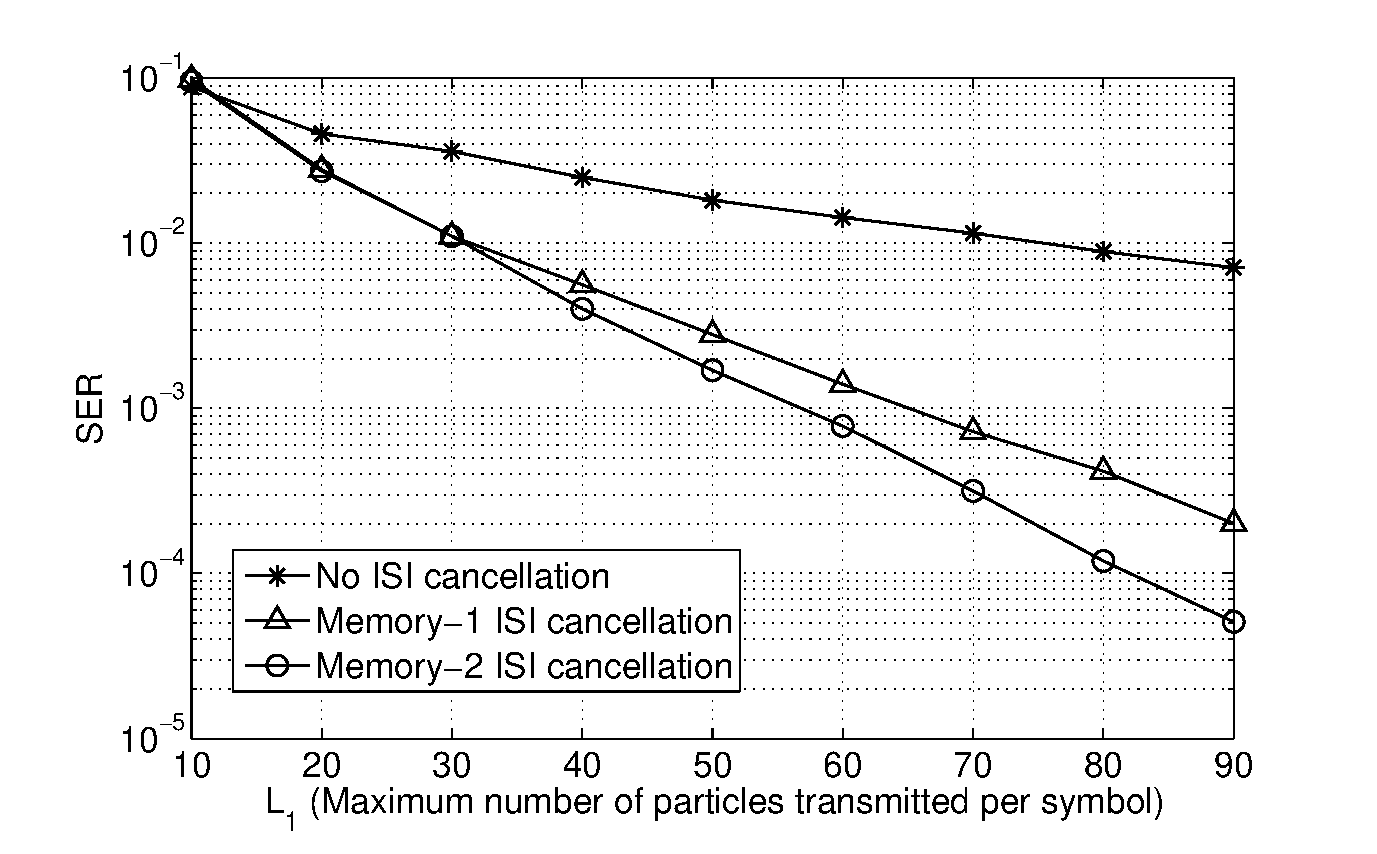
\includegraphics[width=5.5in, keepaspectratio]{QM/binary_ser_0322.eps}
\caption{Binary quantity-based modulation with ISI cancellation.} \label{fig:binary_ser}
\end{figure}

\begin{figure}[htb]
\centering
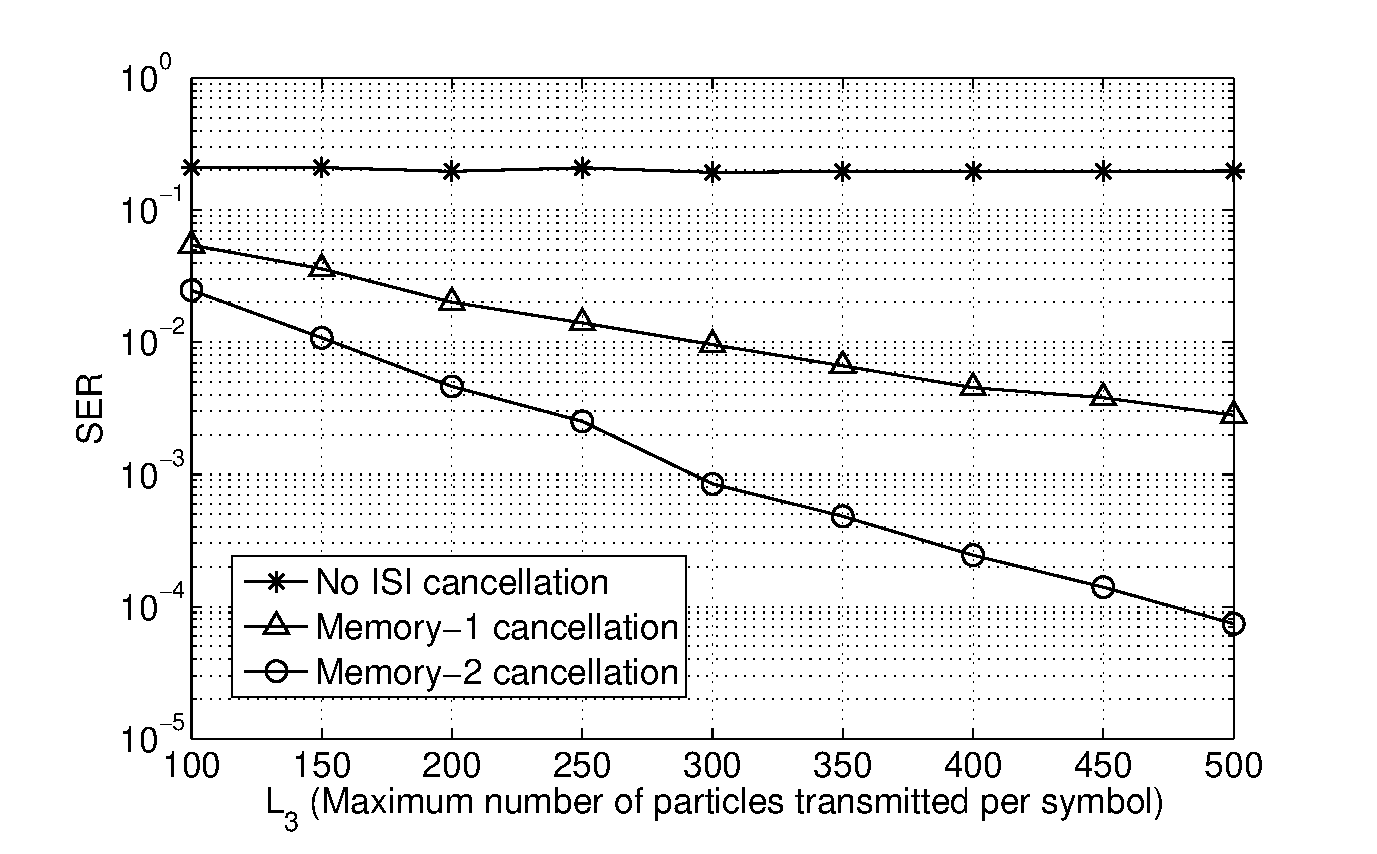
\includegraphics[width=5.5in, keepaspectratio]{QM/4ary_ser_0322.eps}
\caption{Quaternary quantity-based modulation with ISI cancellation.} \label{fig:4ary_ser}
\end{figure}

\subsection{Performance Under Different Duration of Time Slot}
In this subsection, we consider a binary transmission system with and without ISI cancellation for different time slot durations. From Fig.~\ref{fig:timeslots}, we can observe that the SER decreases as the duration $T_s$ increases. In other words, to improve performance, one can increase the duration of the time slot as shown in Fig.~\ref{timeslots}. Although the error rate is already quite acceptable, it can be further improved by the ISI cancellation approach. The improvements is about $10$ times better when $T_s = 10\ s$ and $L_1=70$. Note that when $T_s$ is small, say $T_s = 1\ s$, compared to the expected first-hitting time $d/v$, the error rate increases even if we increase $L_1$ when no cancellation is performed. This is because when $T_s$ is small, molecules tend not to arrive in one symbol time but stay in the background, and that a larger $L_1$ will cause a larger amount of molecules to be in the background and hence larger interference.

\begin{figure}[htb]
\centering
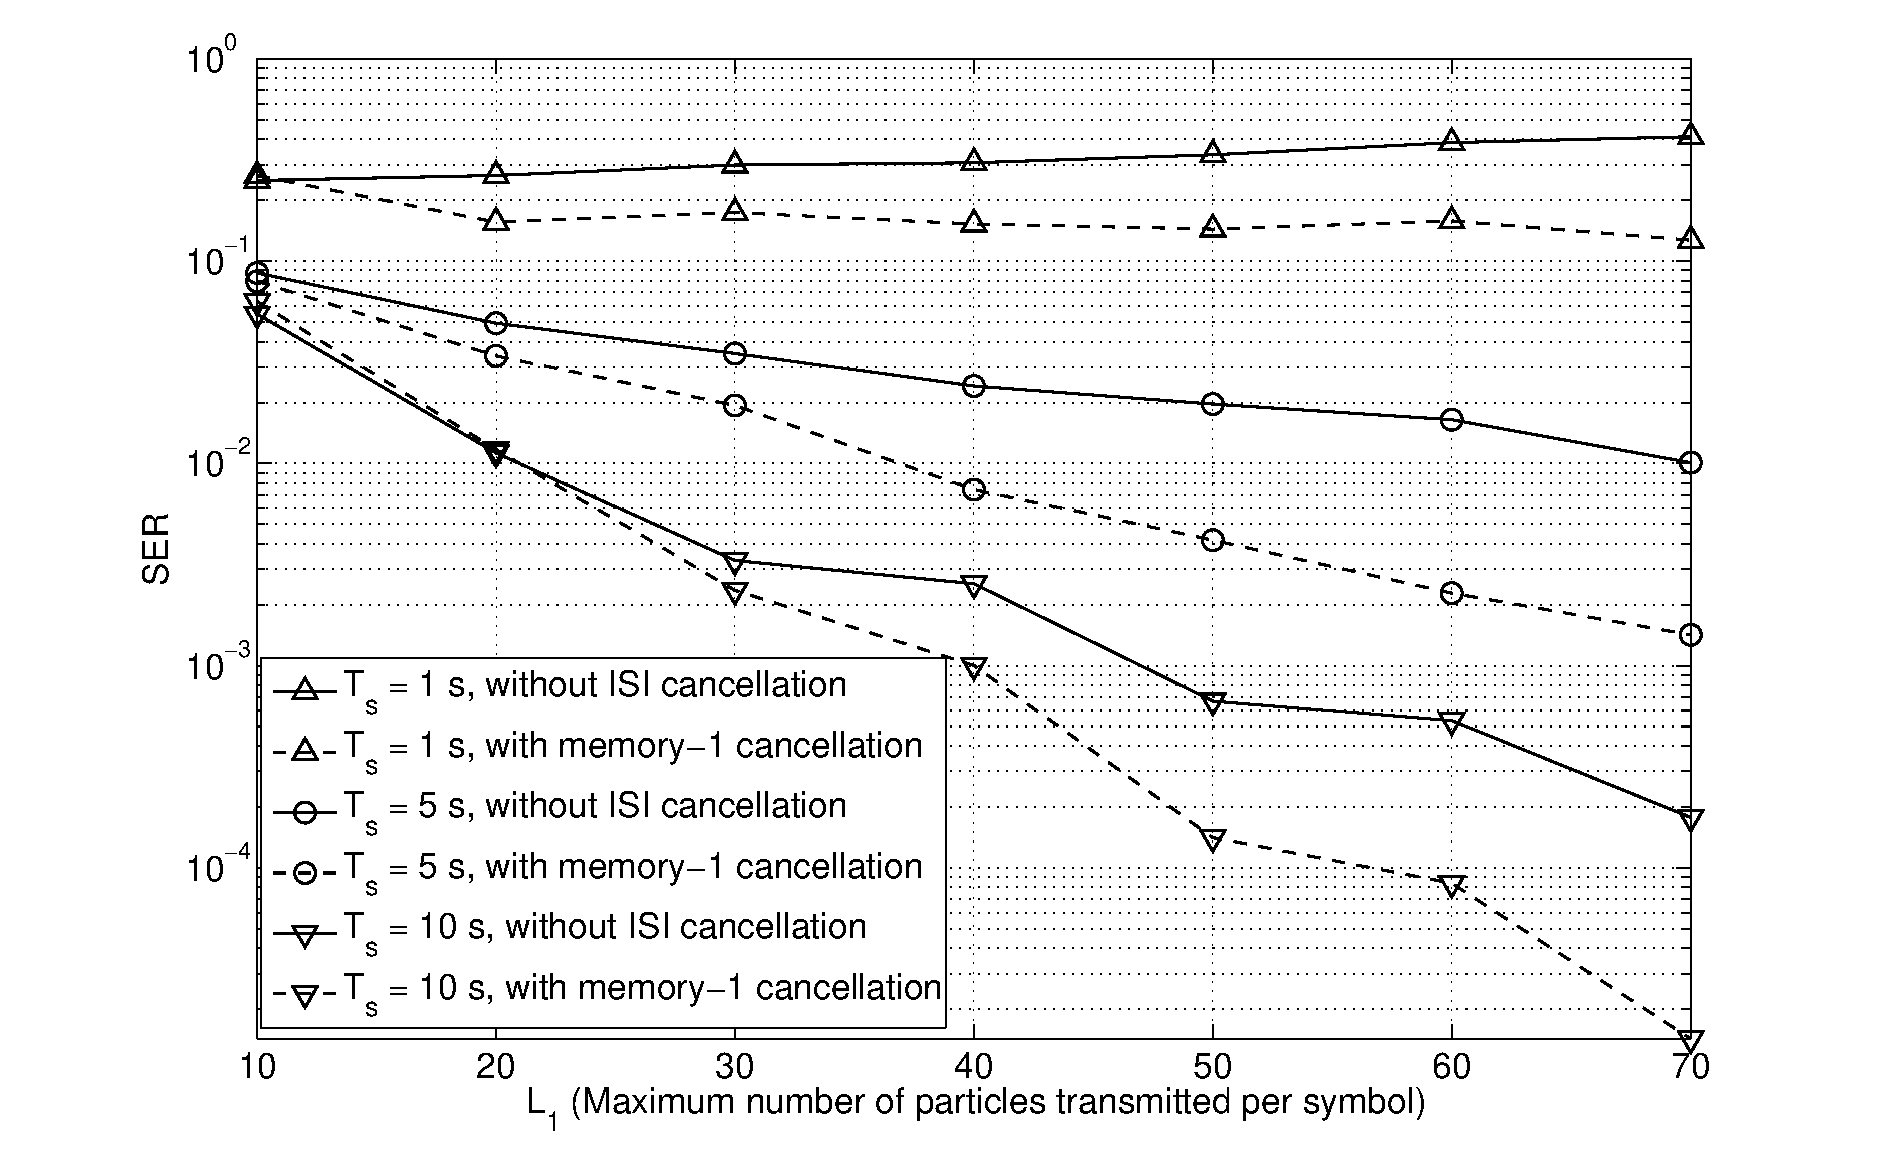
\includegraphics[width=5.5in, keepaspectratio]{QM/timeslots.eps}
\caption{Binary quantity-based modulation with ISI cancellation under different $T_s$.} \label{fig:timeslots}
\end{figure}
